\section{ResNet}
Residuální neuronová síť (ResNet) \cite{ResNet} byla poprvé představena v roce 2015, kdy vyhrála ImageNet Large Scale Visual Recognition Challenge, a svou architekturou silně ovlivnila budoucnost návrhu neuronových sítí.
Síla této neuronové sítě spočívá v tom, že přináší způsob, jak snížit vliv tzv. problému mizejícího gradientu (vanishing gradient problem).
Komplexita neuronových sítí se s každým rokem zvyšuje. Nejvíce se ale konvoluční neuronové sítě rozrůstají do hloubky. Čím je totiž neuronová síť hlubší, tím komplexnější příznaky dokáže extrahovat z původního vstupu a tím složitější funkce dokáže aproximovat.
Čím je ale neuronová síť hlubší, tím více se projevuje problém mizejícího gradientu.
Když je při trénování sítí šířena chyba pomocí algoritmu backpropagation, dochází k tomu, že její vliv je na svrchních vrstvách menší, než na hlubokých. Je-li tedy síť příliš hluboká, tak gradient je na svrchních vrstvách tak malý, že nedochází k přenastavení vah a tyto vrstvy se tedy nijak nemění.
Prohloubení sítě tedy v tomto případě ztrácí smysl a dokonce může mít negativní vliv na její výsledky.
Mělčí neuronové sítě proto mohou při řešení stejného problému dosáhnout mnohem lepších výsledků.

\begin{figure}[h!]
	\centering
	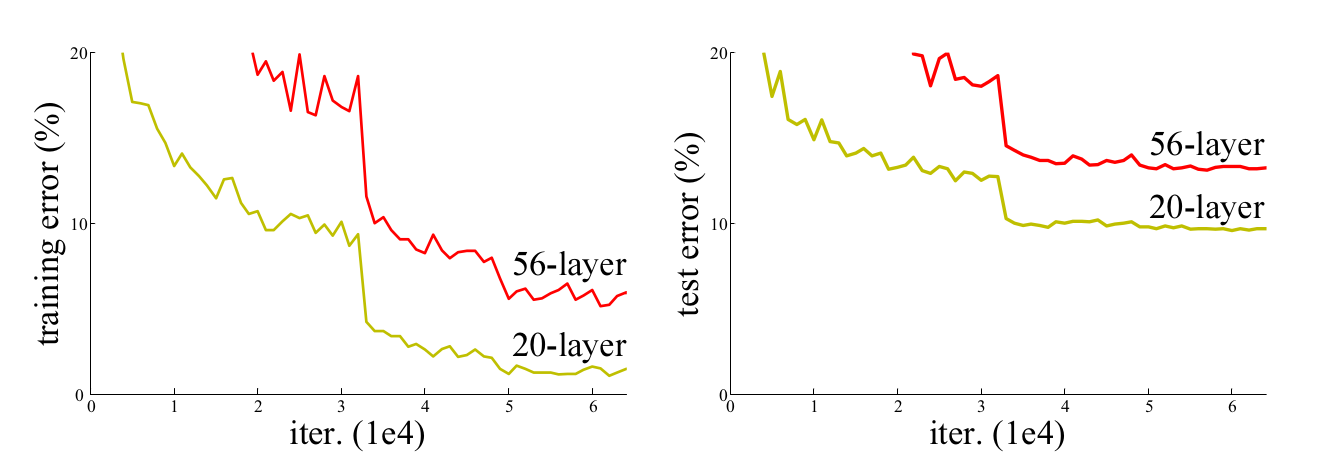
\includegraphics[width=0.7\textwidth]{Figures/solution/vanishing_gradient.png}
	\caption{Porovnání chyby při testování a trénování dvou sítí o hloubce 20 a 56 vrstev určených ke klasifikaci na datasetu CIFAR-10 \cite{ResNet}}
\end{figure}

Síť ResNet je tvořena reziduálními bloky, které jsou podobné VGG blokům \cite{VGG}.
Každý blok obsahuje dvě konvoluce o velikosti 3x3 a každá konvoluce je následovaná normalizací dávky (batch normalization) a aktivační funkcí ReLU.
Co ale reziduální blok přidává je tzv. zkratkové spojení (shortcut connection), které právě pomáhá snižovat vliv mizejícího gradientu.
Zkratkové spojení vezme vstupní hodnoty reziduálního bloku a přidá je k hodnotám před spuštěním druhé aktivační funkce.
V praxi to znamená, že vstupní hodnoty prochází v bloku dvěma cestami, kdy v jedné jsou změněny dvěma konvolucemi, zatímco v druhé se těmto konvolucím vyhnou. Při zpětném šíření chyby sítí se tedy chyba dostane do horních vrstev mnohem rychleji, takže navrhovaná síť může být mnohem hlubší.

\begin{figure}[h!]
	\centering
	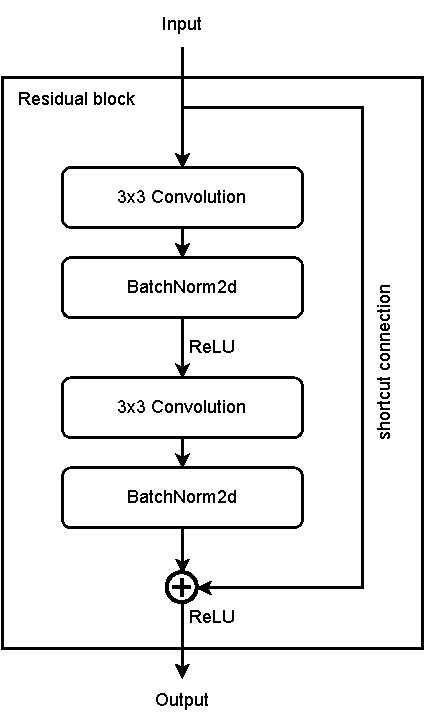
\includegraphics[width=0.3\textwidth]{Figures/solution/residual_block.pdf}
	\caption{struktura reziduálního bloku}
	\label{fig:residual_block}
\end{figure}

Síť ResNet je v navržené síti použita hned na vstupu a jejím cílem je zredukovat dimenzi vstupní sekvence po sobě jdoucích snímků a extrahovat z jednotlivých snímků důležité příznaky, které následně budou využity pro extrakci temporálních informací a konstrukci výsledné hustotní mapy.
Konkrétně je použita síť ResNet18, která obsahuje pouze čtyři reziduální bloky.
Tato varianta byla zvolena kvůli omezenému množství paměti na testovacím stroji.

\endinput